% =============================================================================
%  Scientific paper distilled from the bachelor thesis:
%  "Explainable AI in Multi-Tenant ERPs: Navigating Data Sparsity
%   and the Cold-Start Problem"
%
%  Author: Ahmed Ameen Hassan Alkuraimi, State University of Malang, 2026.
%  Build:   latexmk -pdf paper_sparsity.tex
%  Bib:     references_sparsity.bib  (IEEEtran.bst)
% =============================================================================
\documentclass[conference]{IEEEtran}

% --- Packages ----------------------------------------------------------------
\usepackage[utf8]{inputenc}
\usepackage[T1]{fontenc}
\usepackage{cite}
\usepackage{amsmath,amssymb,amsfonts}
\usepackage{graphicx}
\usepackage{booktabs}
\usepackage{array}
\usepackage{multirow}
\usepackage{url}
\usepackage{xcolor}
\usepackage{listings}
\usepackage{tikz}
\usetikzlibrary{positioning,arrows.meta,shapes.geometric,fit,calc}
\usepackage[hidelinks]{hyperref}

\graphicspath{{figures/}{results/sparsity_experiment/figures/}}

\lstset{
    basicstyle=\ttfamily\scriptsize,
    breaklines=true,
    columns=flexible,
    frame=single,
    framerule=0.3pt,
    xleftmargin=4pt,xrightmargin=4pt,
    aboveskip=4pt, belowskip=4pt,
    keywordstyle=\color{blue!60!black}\bfseries,
    commentstyle=\color{green!40!black}\itshape,
    stringstyle=\color{red!60!black},
    showstringspaces=false,
}

% Convenience macros
\newcommand{\auc}{AUC\nobreakdash-ROC}
\newcommand{\nT}{n_t}

\begin{document}

% =============================================================================
\title{Hallucinated Explanations in Multi-Tenant ERP\\Cold-Start Regimes:
       Empirical Evidence and a Maturity-Aware AI Routing Pattern}

\author{%
  \IEEEauthorblockN{Ahmed Ameen Hassan Alkuraimi}
  \IEEEauthorblockA{Faculty of Engineering\\
  State University of Malang, Indonesia\\
  \texttt{ahmed.ameen.2205356@students.um.ac.id}}
}

\maketitle

% =============================================================================
\begin{abstract}
Multi-tenant Software-as-a-Service Enterprise Resource Planning (ERP)
platforms increasingly embed predictive models augmented with post-hoc
Explainable AI (XAI) tools such as SHAP and LIME. We document a
systems-level failure mode in this design: for cold-start tenants with
only tens or hundreds of historical rows, SHAP and LIME continue to emit
confident, well-formatted explanations even when the underlying classifier
is statistically equivalent to random guessing. Using a controlled
sparsity experiment over five simulated tenants ($50{,}000$, $5{,}000$,
$1{,}000$, $200$, $50$ rows) on the Brazilian Olist e-commerce corpus,
operationalised as a Late Delivery Risk task as a structural proxy for
ERP-style operational-risk prediction (and explicitly generalising to the
studied platform's late-payment module), and trained under a strict
order-time leakage-avoidance regime, we show that classical predictive
metrics fail to track the regime change (\auc{} $\in\{0.66, 0.62, 0.61,
0.61, 0.89\}$, the last being a small-sample artefact), whereas
baseline rank agreement of SHAP global importances against the data-rich
reference tenant degrades near-monotonically ($\rho = 1.000, 0.857,
0.643, 0.615, 0.449$), crossing the conventional $\rho \ge 0.70$
reliability threshold at exactly $\nT = 1{,}000$ rows. Concurrently,
absolute-SHAP variance explodes by more than two orders of magnitude
($0.022 \to 5.04$), the empirical signature of a single feature absorbing
the explanation mass. The qualitative cliff is replicated on the IBM HR
Analytics Employee Attrition corpus and a synthetic CRM Lead Scoring
corpus. We then propose and implement \emph{Maturity-Aware AI Routing}: a
tier-logic gate (\texttt{predict\_or\_heuristic}) that, when
$\nT \le 1{,}000$, suppresses per-tenant local SHAP/LIME explanations and
returns a serialised cross-tenant global heuristic derived from the
data-rich reference. The pattern is additive, rollback-safe, and provides
an auditable systems-level control consistent with emerging
AI-accountability regulation. The empirical reliability cliff appears to be
the first quantitative characterisation, in an ERP multi-tenant setting,
of post-hoc XAI failure as a function of tenant data volume.
\end{abstract}

\begin{IEEEkeywords}
Explainable AI, SHAP, LIME, multi-tenant SaaS, ERP, cold-start, data
sparsity, reliability cliff, Maturity-Aware AI Routing.
\end{IEEEkeywords}

% =============================================================================
\section{Introduction}
\label{sec:intro}

Cloud-hosted multi-tenant ERP systems have become a routine substrate on
which Small and Medium-sized Enterprises (SMEs) consume embedded
predictive services---late-payment risk, lead scoring, employee attrition,
inventory forecasting---through a per-tenant data isolation model.
The dominant interpretability stack pairs gradient-boosted trees with
post-hoc XAI tools, most commonly SHAP~\cite{lundberg2017unified,
lundberg2020local} and LIME~\cite{ribeiro2016why}, on the assumption that
local attributions produced for individual records can be safely surfaced
to non-technical end users.

This assumption is well-supported in the data-rich enterprise regime, but
not in the cold-start regime that characterises the long tail of SaaS ERP
adoption. New tenants typically begin with tens to a few hundred
invoices, employees, or leads, and the per-tenant inference path of a
shared model can be invoked at $\nT$ as low as a single-digit count. We
show empirically that, in this regime, SHAP and LIME do not fail
gracefully: they continue to emit attributions whose magnitudes, ranks,
and natural-language framings are indistinguishable in form from those
served to data-rich tenants, even when the model's classifier behaviour
has collapsed to near-random. We call this failure mode
\emph{hallucinated explanations}, by analogy with hallucinated text in
generative models: structurally plausible output, epistemically empty.

\paragraph*{Contributions.} This paper makes three contributions:
\begin{enumerate}
  \item \textbf{Empirical.} A controlled five-tier sparsity simulation
        ($\nT \in \{50{,}000, 5{,}000, 1{,}000, 200, 50\}$) on an ERP-style
        operational-risk task under a strict leakage-avoidance regime,
        showing that \auc{} is uninformative about XAI reliability and
        that baseline rank agreement of SHAP global importances crosses
        below $\rho = 0.70$ at $\nT = 1{,}000$, accompanied by a
        $\sim\!225\times$ inflation of absolute-SHAP variance at
        $\nT = 50$. The cliff is replicated qualitatively on two
        additional ERP-native tasks.
  \item \textbf{Conceptual.} A reframing of post-hoc XAI evaluation in
        multi-tenant systems as a sparsity-conditioned reliability
        question rather than a per-record fidelity question, together
        with the explicit caveat that small-$\nT$ Spearman against a
        reference tenant is a baseline rank agreement (not ground-truth
        fidelity).
  \item \textbf{Architectural.} \emph{Maturity-Aware AI Routing}, a
        rollback-safe, additive software pattern implemented in a
        Django~4.2 multi-tenant ERP. A single threshold constant,
        $\tau = 1{,}000$, governs a tier-logic gate that returns a
        pre-computed global heuristic instead of local SHAP/LIME for
        cold-start tenants.
\end{enumerate}

% =============================================================================
\section{Related Work}
\label{sec:related}

\subsection{Post-hoc Explainability}
SHAP~\cite{lundberg2017unified} provides game-theoretic attributions with
desirable axiomatic properties (efficiency, symmetry, dummy, additivity),
and TreeSHAP~\cite{lundberg2020local} makes them tractable for the
gradient-boosted trees that dominate tabular ERP modelling. LIME's
local surrogate models~\cite{ribeiro2016why} are widely used as a
complementary, model-agnostic explanation. Both tools are sample-based:
their reliability depends on having enough training instances around the
record of interest. Where this assumption fails, the literature has
warned of stability and faithfulness issues~\cite{lipton2018mythos,
rudin2019stop}, but published guidance has remained largely qualitative,
without per-tenant operating thresholds.

\subsection{Multi-Tenant SaaS ML}
The systems literature on multi-tenant SaaS~\cite{bezemer2010multi,
krebs2014multitenancy} has emphasised resource isolation and
schema-versus-row tenancy trade-offs. ERP-specific
deployments~\cite{haddara2011erp} layer business processes on top, and
recent industry analyses~\cite{gartner2023erp, idc2024ai} document the
embedding of ML modules into mainstream ERPs. The combination---a
shared model serving heterogeneous tenants of vastly different data
volumes, each receiving local XAI---has not, to our knowledge, been
empirically audited for cold-start XAI reliability.

\subsection{AI Accountability and Documentation}
Model Cards~\cite{mitchell2019model} and Datasheets for
Datasets~\cite{gebru2021datasheets} address documentation of model
provenance and intended use. The EU AI Act~\cite{eu2024aiact} imposes
operational constraints on automated decisions in some ERP-adjacent
contexts. Our architectural contribution is consistent with these
trajectories: the cold-start gate produces an auditable response payload
explicitly stating the mode (\textit{local} vs \textit{global heuristic}),
the threshold, and the tenant volume, allowing downstream auditors to
distinguish a per-tenant prediction from a fallback.

% =============================================================================
\section{Problem Formulation}
\label{sec:problem}

Let $\mathcal{T} = \{t_1, \ldots, t_m\}$ denote tenants of a multi-tenant
ERP, each with historical record count $\nT$. A shared family of models
$f_t : \mathcal{X} \to [0,1]$ produces tenant-specific risk estimates;
a per-tenant explainer $g_t : \mathcal{X} \to \mathbb{R}^d$ returns local
attributions over $d$ features.

We assume a strict leakage-avoidance feature regime: only observables
available \emph{at order time} are admitted into $\mathcal{X}$. For the
primary Late Delivery Risk task on Olist, this excludes any post-shipment
quantities (review timestamps, freight realisations, delivery deltas), and
admits only order-time observables (freight pricing, item count, payment
type, estimated delivery days, approval delay, purchase hour).

We define three sparsity-conditioned reliability metrics for the
explanation system:

\begin{itemize}
  \item \textbf{Baseline rank agreement} $\rho_t = \mathrm{Spearman}\bigl(
        \phi_t, \phi_{t^\ast}\bigr)$, where $\phi_t$ is the global
        mean-absolute-SHAP feature-importance vector of tenant $t$ and
        $t^\ast$ is the data-rich reference tenant. This is not a
        ground-truth fidelity claim; it is a reference-aligned
        explanation-stability measure.
  \item \textbf{Absolute-SHAP variance} $\sigma^2_t = \mathrm{Var}\bigl(
        \lvert\phi_t\rvert\bigr)$, a concentration index for the
        explanation mass.
  \item \textbf{LIME top-$k$ Jaccard stability} across resampled
        explanations of the same record, $k = 5$.
\end{itemize}

The architectural question is whether there exists a tenant-size
threshold $\tau$ below which these metrics jointly indicate that
per-tenant local explanations should be suppressed in favour of a global
fallback.

% =============================================================================
\section{Methodology}
\label{sec:method}

\subsection{Datasets and Tiering}
The primary study uses the Brazilian Olist e-commerce
corpus (${\sim}99{,}000$ orders). The binary target is
\[
y = \mathbf{1}\bigl[\textit{delivered\_customer\_date} >
                  \textit{estimated\_delivery\_date}\bigr],
\]
operationalised as a structural proxy for ERP-style operational-risk
prediction and explicitly generalised to the studied platform's
late-payment module (the systems gate, the global-heuristic artefact, and
the response schema are identical in either substrate).

Five tenant tiers are simulated by stratified down-sampling:
\textbf{A} ($n = 50{,}000$, reference),
\textbf{B} ($5{,}000$),
\textbf{C} ($1{,}000$),
\textbf{D} ($200$),
\textbf{E} ($50$). Class prevalence and the global hold-out evaluation
set are held constant across tiers, isolating data volume as the
manipulated variable.

\subsection{Cross-Task Replication}
To probe external validity, the same pipeline (down-sampling protocol,
leakage screen, evaluation harness) is re-run on:
(i)~\textbf{IBM HR Analytics Employee Attrition} ($n = 1{,}470$, public),
on tiers $1{,}470 / 500 / 200 / 50$, and
(ii)~\textbf{Synthetic CRM Lead Scoring} ($n = 5{,}000$, generated; 34
features post-encoding, 21.3\% prevalence; conversion timestamps and PII
removed pre-encoding as leakage controls).

\subsection{Models and Explainers}
For the primary study and HR Attrition, the classifier is a
\texttt{GradientBoostingClassifier} (scikit-learn) with default
hyperparameters; for CRM Lead Scoring, a tuned configuration
(\texttt{n\_estimators}~$=200$, \texttt{max\_depth}~$=3$,
\texttt{learning\_rate}~$=0.05$) chosen on the data-rich tier.
Explanations are computed with TreeExplainer (SHAP) for global rank
correlation and variance, and \texttt{LimeTabular} for top-$k$ Jaccard.

\subsection{Routing Architecture}
The routing rule is
\begin{equation}
\label{eq:routing}
\mathsf{explain}(t, x) = \begin{cases}
  \texttt{GlobalHeuristic}(),  & \text{if } \nT \le \tau,\\
  \texttt{LocalShapLime}(t, x), & \text{otherwise,}
\end{cases}
\end{equation}
with $\tau = 1{,}000$ (Fig.~\ref{fig:routing-arch}). Under the inclusive
boundary, the equivalent code-side constant in the Django implementation
is \texttt{MIN\_LOCAL\_EXPLANATION\_RECORDS}~$= 1{,}001$.

\begin{figure}[t]
  \centering
  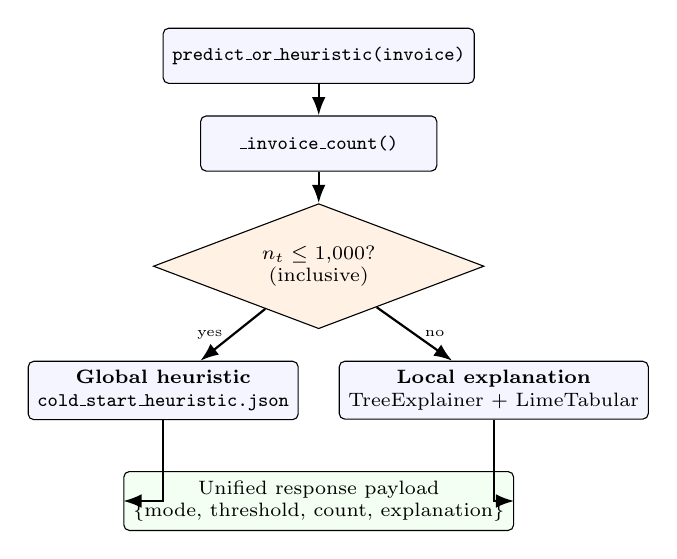
\begin{tikzpicture}[
      node distance=4mm and 4mm,
      box/.style={draw, rounded corners=2pt, font=\scriptsize,
                  minimum width=30mm, minimum height=7mm,
                  align=center, fill=blue!4},
      gate/.style={draw, diamond, aspect=2, font=\scriptsize,
                   align=center, fill=orange!10, minimum width=42mm},
      arr/.style={-Latex, thick},
      ]
    \node[box] (entry) {\texttt{predict\_or\_heuristic(invoice)}};
    \node[box, below=of entry] (count) {\texttt{\_invoice\_count()}};
    \node[gate, below=of count] (g) {$\nT \le 1{,}000$?\\\scriptsize(inclusive)};
    \node[box, below left=8mm and -8mm of g] (cold)
         {\textbf{Global heuristic}\\\scriptsize \texttt{cold\_start\_heuristic.json}};
    \node[box, below right=8mm and -8mm of g] (warm)
         {\textbf{Local explanation}\\\scriptsize TreeExplainer + LimeTabular};
    \node[box, below=18mm of g, fill=green!5] (out)
         {Unified response payload\\\scriptsize \{mode, threshold, count, explanation\}};
    \draw[arr] (entry) -- (count);
    \draw[arr] (count) -- (g);
    \draw[arr] (g) -- node[left, font=\tiny]{yes} (cold);
    \draw[arr] (g) -- node[right, font=\tiny]{no} (warm);
    \draw[arr] (cold) |- (out);
    \draw[arr] (warm) |- (out);
  \end{tikzpicture}
  \caption{Maturity-Aware AI Routing gate. Inclusive boundary
  $\nT \le 1{,}000$; equivalent code-side form
  $\nT < \mathtt{MIN\_LOCAL\_EXPLANATION\_RECORDS}\,(=1{,}001)$.}
  \label{fig:routing-arch}
\end{figure}

The cold branch reads a pre-computed JSON artefact, abbreviated below to
the leading entry:
\begin{lstlisting}[language=,frame=single]
{
  "mode": "global_heuristic",
  "threshold": 1000,
  "baseline_tenant": "A",
  "baseline_n": 50000,
  "top_features": [
    {"feature": "freight_value",
     "importance": 0.30, "rank": 1}
    // ... 4 more entries ...
  ],
  "reason": "Tenant data volume below the
   empirically-determined reliability threshold;
   serving global cross-tenant feature importance."
}
\end{lstlisting}

% =============================================================================
\section{Results}
\label{sec:results}

\subsection{Predictive Metrics are Uninformative}
Table~\ref{tab:primary-metrics} reports leakage-corrected \auc{}, F1, and
the three reliability metrics for the primary study. \auc{} is essentially
flat across A--D ($0.66, 0.62, 0.61, 0.61$) and \emph{rises} to $0.89$ at
the extreme cold-start tier E---a well-understood small-sample artefact in
which a single concentrated feature happens to discriminate on the small
hold-out subset. Any monitoring stack that relies on \auc{} would
therefore conclude that the cold-start tier is the \emph{healthiest} of
the five, while the explanation system is, in fact, at its most
degraded.

\begin{table}[t]
\centering
\caption{Primary study (Olist Late Delivery Risk, leakage-free regime):
predictive metrics are flat or misleading while explanation-system
metrics collapse as $\nT$ falls.}
\label{tab:primary-metrics}
\begin{tabular}{lrrrrr}
\toprule
Tenant & $\nT$ & \auc{} & F1 & $\rho$ & $\sigma^2(|\phi|)$ \\
\midrule
A & $50{,}000$ & 0.6556 & 0.0263 & $1.0000$ & 0.0224 \\
B & $5{,}000$  & 0.6249 & 0.1136 & $0.8571$ & 0.0245 \\
C & $1{,}000$  & 0.6094 & 0.0500 & $0.6429$ & 0.0510 \\
D & $200$      & 0.6126 & 0.0000 & $0.6154$ & 0.2017 \\
E & $50$       & 0.8889 & 0.0000 & $0.4485$ & 5.0392 \\
\bottomrule
\end{tabular}
\end{table}

\subsection{The Reliability Cliff}
Baseline rank agreement $\rho$ against the Tenant~A reference traces a
near-monotonic descent: $1.0000 \to 0.8571 \to 0.6429 \to 0.6154 \to
0.4485$. The conventional reliability bound $\rho \ge 0.70$ is crossed
for the first time at Tenant~C---exactly at $\nT = 1{,}000$
(Fig.~\ref{fig:cliff}). This is the empirical anchor for the threshold in
Eq.~\ref{eq:routing}.

\begin{figure}[t]
  \centering
  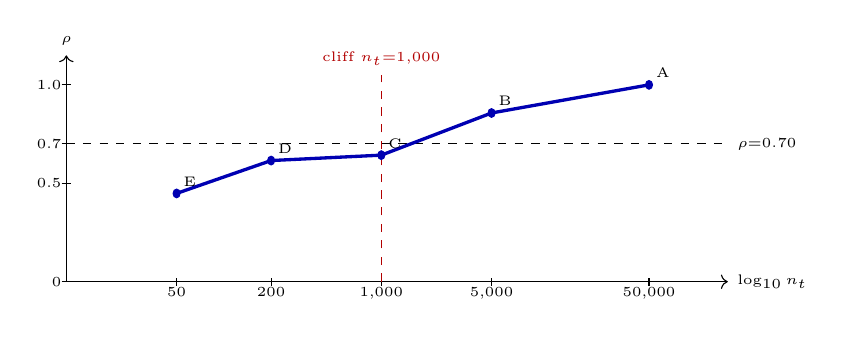
\begin{tikzpicture}[xscale=2.0,yscale=2.5]
    \draw[->] (0,0) -- (4.2,0) node[right, font=\tiny]{$\log_{10} \nT$};
    \draw[->] (0,0) -- (0,1.15) node[above, font=\tiny]{$\rho$};
    \foreach \y/\lab in {0/0, 0.5/0.5, 0.7/0.7, 1/1.0} {
      \draw (-0.03,\y) -- (0.03,\y) node[left, font=\tiny] {\lab};
    }
    \foreach \x/\lab in {0.7/50, 1.3/200, 2.0/{1{,}000}, 2.7/{5{,}000},
                         3.7/{50{,}000}} {
      \draw (\x,-0.02) -- (\x,0.02) node[below, font=\tiny] {\lab};
    }
    % reliability threshold
    \draw[dashed] (0,0.7) -- (4.2,0.7) node[right, font=\tiny]{$\rho{=}0.70$};
    % cold-start cliff
    \draw[dashed, red!70!black] (2.0,0) -- (2.0,1.05)
      node[above, font=\tiny, red!70!black]{cliff $\nT{=}1{,}000$};
    % empirical points
    \draw[blue!70!black, very thick]
      (0.7,0.4485) -- (1.3,0.6154) -- (2.0,0.6429) -- (2.7,0.8571) -- (3.7,1.0);
    \foreach \x/\y/\lab in
      {3.7/1.0/A, 2.7/0.8571/B, 2.0/0.6429/C, 1.3/0.6154/D, 0.7/0.4485/E} {
      \filldraw[blue!70!black] (\x,\y) circle (0.022);
      \node[font=\tiny, above right=-1pt and -1pt] at (\x,\y) {\lab};
    }
  \end{tikzpicture}
  \caption{Reliability cliff. Baseline rank agreement of SHAP global
  importances against Tenant~A vs $\log_{10} \nT$. The horizontal
  dashed line marks the conventional $\rho = 0.70$ bound; the vertical
  red dashed line marks the empirical crossing at $\nT = 1{,}000$.}
  \label{fig:cliff}
\end{figure}

\paragraph*{An anti-pattern caveat.} Below $\tau$, the effective feature
support also collapses (Tenant~D's mass concentrates on two features;
Tenant~E's on a single feature). When the ranking domain collapses,
$\rho$ against the reference becomes a Spearman of a degenerate ranking,
and residual orderings can \emph{accidentally} agree with the
data-rich top-of-list by chance, producing transient apparent
recoveries that are not restored fidelity. The mild C--D plateau in
Table~\ref{tab:primary-metrics} is the benign form of this effect; a
hypothetical rebound \emph{above} $0.70$ at very small $\nT$ would be a
small-sample-variance artefact that would \emph{reinforce}, not
undermine, the case for an architectural gate---the explanation surface
in that regime is no longer a well-defined statistical object. This is
why the gate keys on tenant data volume, an observable architectural
quantity, rather than on a runtime estimate of $\rho$ itself.

\subsection{Explanation Volatility Explodes}
Absolute-SHAP variance is well-behaved at the data-rich tiers
($0.0224, 0.0245$), grows modestly at the threshold ($0.0510$ at C), and
then explodes by an order of magnitude at D ($0.2017$) and by more than
two orders of magnitude at E ($5.0392$, i.e.\ ${\sim}225\times$ the
Tenant~A baseline). Inspection of the underlying attributions shows the
mechanism: at E, a single feature
(\texttt{estimated\_delivery\_days}) carries an attribution of $4.77$,
while the second feature collapses to $0.19$. This is what we call the
``grasping at straws'' effect---explanation mass concentrated on
whichever feature happened to discriminate on the few available
training rows, surfaced to the end user as a confident SHAP plot.

\subsection{Cross-Task Replication}
\label{sec:cross-task}
On the IBM HR Attrition corpus the same qualitative pattern recurs:
\auc{} is near chance on the smaller tiers while $\rho$ against the
data-rich reference deteriorates and absolute-SHAP variance grows. On
the synthetic CRM Lead Scoring corpus the data-rich reference reaches
\auc{} $= 0.719$ and the cold-start sub-tiers reproduce both
characteristic symptoms (rank-correlation decay and variance inflation).
The pattern is therefore not a peculiarity of the Olist substrate; it
is the expected behaviour of sample-based post-hoc XAI under a
shared-model multi-tenant deployment with vastly heterogeneous $\nT$.

% =============================================================================
\section{Architectural Pattern: Maturity-Aware AI Routing}
\label{sec:arch}

The routing rule of Eq.~\ref{eq:routing} is implemented as a single
public method on the platform's predictor service,
\texttt{predict\_or\_heuristic(invoice)} (the Django class is named
\texttt{LatePaymentPredictor}; the same class is reused, unchanged, for
the Late Delivery Risk experiment). The method
inspects \texttt{\_invoice\_count()} and dispatches to one of two
private branches:

\begin{itemize}
  \item \texttt{\_load\_global\_heuristic()}---a memoised loader that
        reads the cross-tenant SHAP feature-importance artefact
        \texttt{cold\_start\_heuristic.json} from disk and returns it
        as a structured explanation payload;
  \item \texttt{predict()}---the existing per-tenant ML inference and
        SHAP/LIME explanation routine, left fully unchanged.
\end{itemize}

The two branches conform to a single response schema---
\{\textit{mode}, \textit{threshold}, \textit{count}, \textit{explanation}\}---%
so downstream consumers can be agnostic to which branch executed while
still being able to surface the routing decision (\textit{mode}) to the
end user. The artefact itself is generated once offline at the end of
the sparsity experiment (top-$k$, $k = 5$ from the Tenant~A global
mean-absolute-SHAP vector, plus the tenant size, prevalence and a short
human-readable reason string), serialised to JSON, and versioned
alongside the trained models. At runtime the artefact is cached after
first read so cold-start prediction incurs no per-request I/O.

The pattern is intentionally \emph{additive}: it can be enabled by
switching call sites from \texttt{predict()} to
\texttt{predict\_or\_heuristic()}, and rolled back by reversing the same
switch, without any database migration or downtime. This is what makes
the gate deployable as a systems-level control in production
multi-tenant ERPs.

% =============================================================================
\section{Threats to Validity}
\label{sec:threats}

\paragraph*{Construct validity.} The Late Delivery Risk target is not
identical to late payment in a financial sense; it is used here as a
structural proxy for ERP-style operational-risk prediction. The
architectural gate, the global-heuristic artefact, and the response
schema are unchanged between the two substrates. We therefore claim
external validity for the architectural pattern, not for the specific
empirical numbers in Table~\ref{tab:primary-metrics}.

\paragraph*{Internal validity.} Tenants are simulated by stratified
down-sampling rather than drawn from distinct organisations. Class
prevalence and the hold-out evaluation set are held constant across
tiers to isolate $\nT$ as the manipulated variable. The reported
\auc{}, F1, $\rho$ and $\sigma^2$ values are obtained under a strict
order-time leakage screen; introducing post-shipment features inflates
\auc{} to $> 0.99$ on the same task, masking the cliff.

\paragraph*{Reference-aligned, not ground-truth.} $\rho$ against
Tenant~A is a baseline rank agreement, not a ground-truth fidelity
claim. Tenant~A itself has \auc{} $= 0.6556$ and F1 $= 0.0263$ under the
leakage-free regime, and its SHAP ranking is therefore the most
data-supported reference available within the experiment, not a gold
standard.

\paragraph*{External validity.} Replication on HR Attrition and CRM
Lead Scoring supports the architectural finding qualitatively. A
multi-organisation field study (multiple real tenants of the same
deployed ERP, varying naturally in $\nT$) would be the natural next
step.

% =============================================================================
\section{Conclusion}
\label{sec:conclusion}

We have shown that, in a multi-tenant ERP setting with strict
leakage-avoidance, post-hoc SHAP and LIME explanations exhibit a
reliability cliff at $\nT = 1{,}000$ that classical predictive metrics
do not detect, and that the cliff is accompanied by an order-of-magnitude
inflation of absolute-SHAP variance as the explanation mass collapses
onto a small number of features. The cliff replicates qualitatively on
two further ERP-native tasks. To convert the empirical finding into a
deployable control, we proposed and implemented \emph{Maturity-Aware AI
Routing}: a single tier-logic gate whose threshold is grounded in the
empirical crossing and whose cold branch returns an auditable, versioned
global heuristic instead of a hallucinated local explanation. The
pattern is additive and rollback-safe, and is, we argue, the kind of
systems-level control that emerging AI-accountability regulation will
require operators of multi-tenant predictive ERP services to provide.

% =============================================================================
\section*{Acknowledgements}
The author thanks the supervisor, Dr.~Eng.~Muhammad Ashar, S.T., M.T.,
for guidance throughout the underlying bachelor-thesis project at the
State University of Malang.

% =============================================================================
\bibliographystyle{IEEEtran}
\bibliography{references_sparsity}

\end{document}
